\documentclass[a4paper, 11pt]{article}
\usepackage[english]{babel}
\usepackage{parskip}
\usepackage{graphicx}
\usepackage{listings}
\usepackage{color}
\definecolor{dkgreen}{rgb}{0,0.6,0}
\definecolor{gray}{rgb}{0.5,0.5,0.5}
\definecolor{mauve}{rgb}{0.58,0,0.82}

\lstset{frame=tb,
  language=PHP,
  aboveskip=3mm,
  belowskip=3mm,
  showstringspaces=false,
  columns=flexible,
  basicstyle={\small\ttfamily},
  numbers=left,
  numberstyle=\tiny\color{gray},
  keywordstyle=\color{blue},
  commentstyle=\color{dkgreen},
  stringstyle=\color{mauve},
  breaklines=true,
  breakatwhitespace=true,
  tabsize=3
}
\newcommand{\head}[1]{\textnormal{\textbf{#1}}}
\begin{document}
\title{PaxListConverter}
\author{EU-Maritime}
\maketitle

\section{Dedication}
This work is dedicated to friends and foes, students and teachers, bosses and clients who have triggered my curiosity during many years. They were the true motor of this work, they provided the motivation for the hard work needed to produce this work. I did enjoy the challenge and ask them to find here the reward they have merited. Thank you folks!

\section{The purpose}
\head{
Some obstacles can't be jumped and the best way to handle those is to walk around.
}

Trying to find a unique format and hoping the rest of the world to embrace it looks like an utopia to me. I think the world uses different ways to communicate, in this particular case, the list of passengers, crew and stowaway aboard a ship to the port of call (=destination). What I will explain here is not only usable to the maritime world, it's true for all situation where a single format can't be forced.

The convention (here, in this sample application) is that the data needed is a sort of table where the columns hold the different data fields and where the lines holds data of a single person. The very first line of this table hold the title of the column. The order of the columns is not (or should'nt be) irrelevant, nor the order of the lines. Mixing the passengers and the crew doesn't matter, and if it does the it is the Filters responsability.  Quite standard I believe. Here is a small list of my passengers and crew.
\begin{center}
\begin{tabular}{|c|l|l|l|}
\hline 
\multicolumn{4}{|c|}{PaxList}\\
\hline \hline
CPS & FirstName & LastName & BirthDate \\
\hline
S & Harry & Potter & 1999-12-31\\
P & Gildor & Inglorion & 1998-11-30\\
C & Grima & Wormthongue & 1997-10-29\\
C & Barliman & Butterbur & 1996-09-28\\
P & Bilbo & Baggins & 1995-08-27\\
\hline
\end{tabular}
\end{center}
There is one little thing that hurts me. Why should the birthdate be written in the YYYY-MM-DD format and not my preferred format (or just because a have the birthdates in another format), like MM/DD/YY? Well I can, like this, where date columns names are followed by an underscore and the format.
\begin{center}
\begin{tabular}{|c|l|l|r|}
\hline 
\multicolumn{4}{|c|}{PaxList}\\
\hline \hline
CPS & FirstName & LastName & BirthDate\textunderscore MM/DD/YY\\
\hline
S & Harry & Potter & 12/31/99\\
P & Gildor & Inglorion & 11/30/98\\
C & Grima & Wormthongue & 10/29/97\\
C & Barliman & Butterbur & 09/28/96\\
P & Bilbo & Baggins & 08/27/95\\
\hline
\end{tabular}
\end{center}
All the formats I support can be found in the class variable \textbf{\textdollar dateFormat} of \textbf{PassengersFilter}.

\section{The Design Pattern}
\head{Don't reinvent the wheel.}

I was largely inspired by \textbf{Mattias Noback}'s book \textbf{Principes of Package Design} publish by \textbf{LeanPub} and his excellent talk in the PHP devroom at FOSDEM 2015. You will find a lot of similarities between his book and the code here. The most important think is to apply an existent pattern, not to find new one's. So here is the implementation I made, three times: once for the \texttt{Decoder}, once for the \texttt{Filter} and finally for the \texttt{Encoder}. I will use the \texttt{Decoder} to read a file containing the \textit{PassengerList} from different file formats, I will use the \texttt{Filter} to verify, adapt, move, ... the content and finally I will output the filtered content using an \texttt{Encoder}.

For example I will use a \texttt{ExcelDecoder} to read a Excel sheet, compute the dates with the \texttt{Filter} and I will output the content in HTML using the \texttt{HtmlEncoder}, in Json using the \texttt{JsonDecoder} and in Xml using the \texttt{XmlDecoder}. Of course, in reality, you, probably, want to output in only one format.

The files needed to implement the Decoder part are:
\begin{itemize}
\item DecoderInterface (see listing ~\ref{lst:interface})
\item DecoderInterfaceFactory (see listing ~\ref{lst:interfacefactory})
\item DecoderFactory (see listing ~\ref{lst:factory})
\item GenericDecoder (see listing ~\ref{lst:generic})
\end{itemize}
and your implementation should contain:
\begin{itemize}
\item CsvDecoder (to decode a comma separated file, see listing ~\ref{lst:concrete})
\end{itemize}
and repeat this for \texttt{Filter} and for \texttt{Encoder} (if you need them).
\subsection{Decoder}
\subsubsection{Interface}
Typically the \texttt{DecoderInterface} contains:
 \label{lst:interface}
\begin{lstlisting}
<?php
interface DecoderInterface
{
	/**
	 * @param string $format
	 * @return array of dict $data
	 */
	public function decode(/* string */$format);
}
\end{lstlisting}
and will be used by the specific \texttt{Decoder} (here the \texttt{CsvDecoder}).
 
\subsubsection{FactoryInterface}
Typically the \texttt{DecoderFactoryInterface} contains:
\label{lst:interfacefactory}
\begin{lstlisting}
<?php
interface DecoderFactoryInterface
{
	/**
	 * Create a decoder for the given format
	 *
	 * @param string $format
	 * @return DecoderInterface concrete Class defined by $format
	 */
	public function createForFormat(/* string */$format);
}
\end{lstlisting}
in this way we can satisfy to the S\underline{O}LID principle : 'open for extension, closed for modification'.
\subsubsection{Factory}
\label{lst:factory}
\begin{lstlisting}
<?php
require_once 'Decoder/DecoderFactoryInterface.php';

class DecoderFactory implements DecoderFactoryInterface
{
	private $factories = [];

	/**
	 * Register a callable that returns an instance of DecoderInterface for the given format
	 * @param string   $format
	 * @param callable $factory
	 */
	public function addDecoderFactory(/* string */$format, callable $factory)
	{
		$this->factories[$format] = $factory;
	}

	/**
	 * @param string $format
	 * @return DecoderInterface concrete Class defined by $format
	 */
	public function createForFormat (/* string */$format)
	{
		$factory = $this->factories[$format];
		
		return $factory();
	}
}
\end{lstlisting}

\subsubsection{Generic}
\label{lst:generic}
The \texttt{genericDecoder} is used to call any decoder passed as a parameter in the constructor
\begin{lstlisting}
<?php
class GenericDecoder
{
	private $decoderFactory;

	/**
	 * GenericDecoder constructor.
	 * @param DecoderFactory $decoderFactory
	 */
	public function __construct(/*DecoderFactory*/ $params)
	{
		$this->decoderFactory = $params;
	}

	/**
	 * @param array $data
	 * @param string $format
	 * @return mixed
	 */
	public function decodeToFormat (array $data, /* string */$format)
	{
		$decoder = $this->decoderFactory->createForFormat($format);
		return = $decoder->decode($data);
	}
}

\end{lstlisting}

\subsubsection{A concrete implementation : the CsvDecoder}
One of the simplest decoder to program.
\label{lst:concrete}
\begin{lstlisting}
<?php
require_once LIBRARIES.'Decoder/DecoderInterface.php';

class CsvDecoder implements DecoderInterface
{
	/**
	 * @param string $data
	 * @return array of dict
	 */
	public function decode(/* string */$dataFile)
	{
		$dataLine = [];
		$handle = fopen($dataFile, 'rt');
		if ($handle) {
			//read first line
			$keys = fgetcsv($handle);
			//read data lines
			while ($nextLine = fgetcsv($handle)) {
				$dataLine[] = array_combine($keys, $nextLine);
			}
		}
		return $dataLine;
	}
}
\end{lstlisting}
\subsection{Filter}
Here a my \texttt{PassengersFilter}, it could help to understand in which conditions one could use \texttt{Filter} to improve the system, without changing the code of the core (which is close for modifications). 
\begin{lstlisting}
<?php
class PassengersFilter implements FilterInterface
{
	public $fields;
	public $dateFormats;

	public function __construct()
	{
		$this->fields = [
		    'CPS'           => 'CPS',   // for C rew, P ax, S towaways
		    'FIRSTNAME'     => 'CP',
		    'LASTNAME'      => 'CP',
		    'NATIONALITY'   => 'CP',
		    'RANKORRATING'  => 'C',
		    'TYPEOFID'      => 'CP',
		    'SERIALNRID'    => 'CP',
		    'SERIALNRVISA'  => 'P',     //necessary ev. empty
		    'EXPDATE_'      => 'CP',
		    'BIRTHDATE_'    => 'CP',
		    'PLACEOFBIRTH'  => 'CP',
		    'EMBARKATION'   => 'P',
		    'DISEMBARKATION'=> 'P',
		];
		$this->dateFormats = [
			'YYYY-MM-DD' => 'Y-m-d',  'YY-MM-DD' => 'y-m-d',
			'YYYY/MM/DD' => 'Y/m/d',  'YY/MM/DD' => 'y/m/d',
			'DD-MM-YYYY' => 'd-m-Y',  'DD-MM-YY' => 'd-m-y',
			'DD/MM/YYYY' => 'd/m/Y',  'DD/MM/YY' => 'd/m/y',
			'MM-DD-YYYY' => 'm-d-Y',  'MM-DD-YY' => 'm-d-y',
			'MM/DD/YYYY' => 'm/d/Y',  'MM/DD/YY' => 'm/d/y',
			'EXCEL'      => 'EXCEL',
		];
	}

	/**
	 * @param array of dict $data
	 * @return array 
	 */
	public function filter (array $data)
	{
		//read first line
		$firstLine = $data[0];
		//check if the required fields are present
		$foundFormat = [];
		$missingPFields = $this->findMissingFields('P', $firstLine, $foundFormat);
		$missingCFields = $this->findMissingFields('C', $firstLine, $foundFormat);
		print_r($foundFormat);
		echo '<br/>missing fields for P ';
		print_r($missingPFields);
		echo '<br/>missing fields for C ';
		print_r($missingCFields);

		$filteredC = $this->prepareData('C', $data);
		$filteredP = $this->prepareData('P', $data);
		
		return array_merge($filteredC, $filteredP);
	}

	/**
	 * @param string $cat
	 * @param array of dict $data
	 * @return array
	 */
	private function prepareData(/* string */$cat, array $data)
	{
		$dataOut = [];
		foreach ($data as $row){
			if ($row['CPS'] != $cat)
				continue;

			$rowOut = [];
			foreach($row as $key => $val)
			{
				$key = strtoupper($key);
				$pos = strpos($key, '_');
				if ($pos !== false){
					$fmt = substr($key, $pos + 1);
					$fmt = $this->dateFormats[$fmt];
					$key = substr($key, 0, $pos);
				}
				switch ($key){
					case 'EXPDATE':
					case 'BIRTHDATE':
						if ($fmt == 'EXCEL'){
							$rowOut[$key] = $val;
						} else {
							$date = DateTime::createFromFormat($fmt, $val);
							$rowOut[$key] = $date->format('Y-m-d');
						}
					break;
					default:
						$rowOut[$key] = strtoupper($val);
				}
			}
			$dataOut[] = $rowOut;
		}
		return $dataOut;
	}

	/**
	 * @param string $cat
	 * @return array
	 */
	private function getFieldsFor(/* string */$cat)
	{
		$fields = [];
		foreach ($this->fields as $k => $v){
			if (strpos($v, $cat) !== false){
				$fields[] = $k;
			}
		}

		return $fields;
	}

	/**
	 * @param string $cat
	 * @param string $firstLine
	 * @param &array $foundFormat
	 * @return array
	 */
	private function findMissingFields($cat, $firstLine, &$foundFormat)
	{
		$mandatory = $this->getFieldsFor($cat);
		$keys = array_keys($firstLine);
		foreach($keys as &$k){
			$k = strtoupper($k);
			$pos = strpos($k, '_');
			if ($pos !== false){
				$dateFormat = substr($k, $pos+1);
				$k = substr($k, 0, $pos+1);
				$foundFormat[$k] = $this->dateFormats[$dateFormat];
			}
		}
		asort($keys);
		asort($mandatory);
		$result = array_diff($mandatory, $keys);
		return $result;
	}
}
\end{lstlisting}
I must admit that the lines 46 to 51 are not at the right place and should be moved out of the class and put in a class with output responsibilities (I still have some work to do).
\subsection{Encoder}
I want to show the \texttt{JsonEncoder}, 
\begin{lstlisting}
<?php
class JsonEncoder implements EncoderInterface
{
	/**
	 * @param array of dict $data
	 * @return string
	 */
	public function encode(array $data)
	{
		$data = json_encode($data);
		$data = str_replace('\"', '', $data);
		
		return $data;
	}
}
\end{lstlisting}
PHP is so kind to do nearly the whole job ;-)
\section{Putting everything together}
The \texttt{Load} class is the main thing, it is a \texttt{CI\textunderscore Controller} class from CodeIgniter 3.0.6. Since it takes over the 200 lines of code, I want to highlight only some part of it. The complete code is available, you'll have it all.
How to call the stuff from your browser.
\begin{itemize}
\item Install PHP (\textgreater= 5.4).
\item Install CodeIgniter (\textgreater = 3.0.6).
\item Run composer to get the package PHPOffice/phpExcel.
\item Install all the code included here.
\item if you don't have a HTTP server type on the command line:

 \texttt{php -S localhost:8080 path\textunderscore to\textunderscore  index.php}
\item in your browser : localhost:8080/PaxListConverter/Load.
\item you should see something like the figure ~\ref{fig:before}.
\item Choose a file from the folder \texttt{doc}.
\item Click the button \texttt{Upload}.
\item you should see something like the figure ~\ref{fig:after}.
\item enjoy.
\end{itemize}
\section{Figures}
\subsection{Figure before upload}
\label{fig:before}
The figure when you \texttt{Browse} to PaxList in Excel and before you click \texttt{Upload File}.

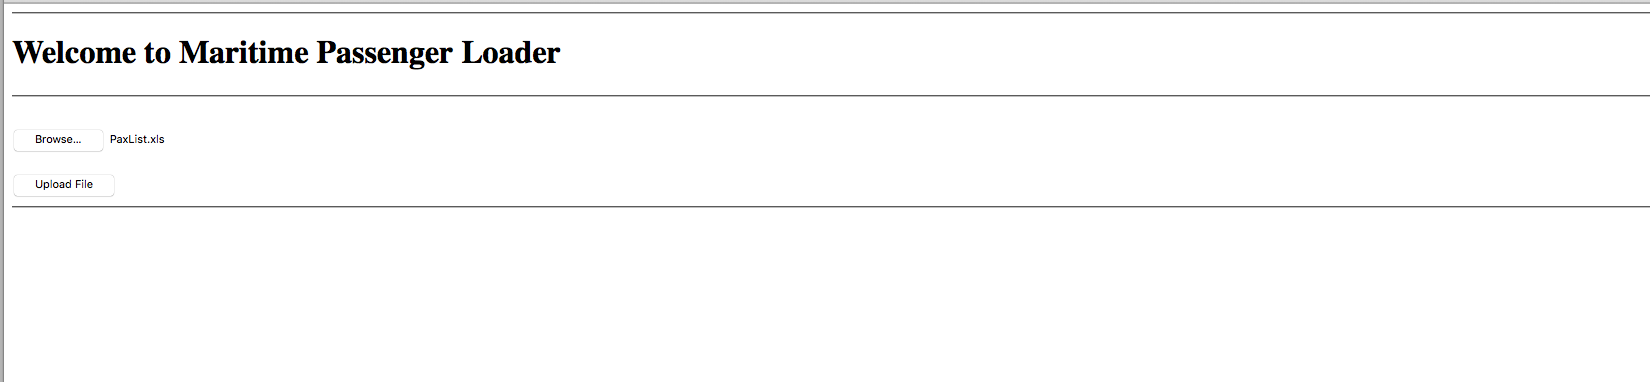
\includegraphics{figures/before}

\subsection{Figure after upload}
\label{fig:after}
Once you click \texttt{Upload File} you get this figure with:
\begin{itemize}
\item A line with information about the date formats.
\item A line with missing mandatory columns for Passengers.
\item A line with missing mandatory columns for Crew.
\item The title 'Welcome to Maritime Passenger Loader'.
\item The section with \texttt{Browse} and \texttt{Upload File} buttons.
\item A section about the file being read containing error, name, type, size and allowed.
\item A Section HTML, being the result of the \texttt{HtmlEncoder}.
\item A section XML, being the html version of the result of \texttt{XmlEncoder}.
\item A line telling you the name of the xml file create by \texttt{XmlEncoder}.
\item The same for JSON, in html and as a file.
\end{itemize}
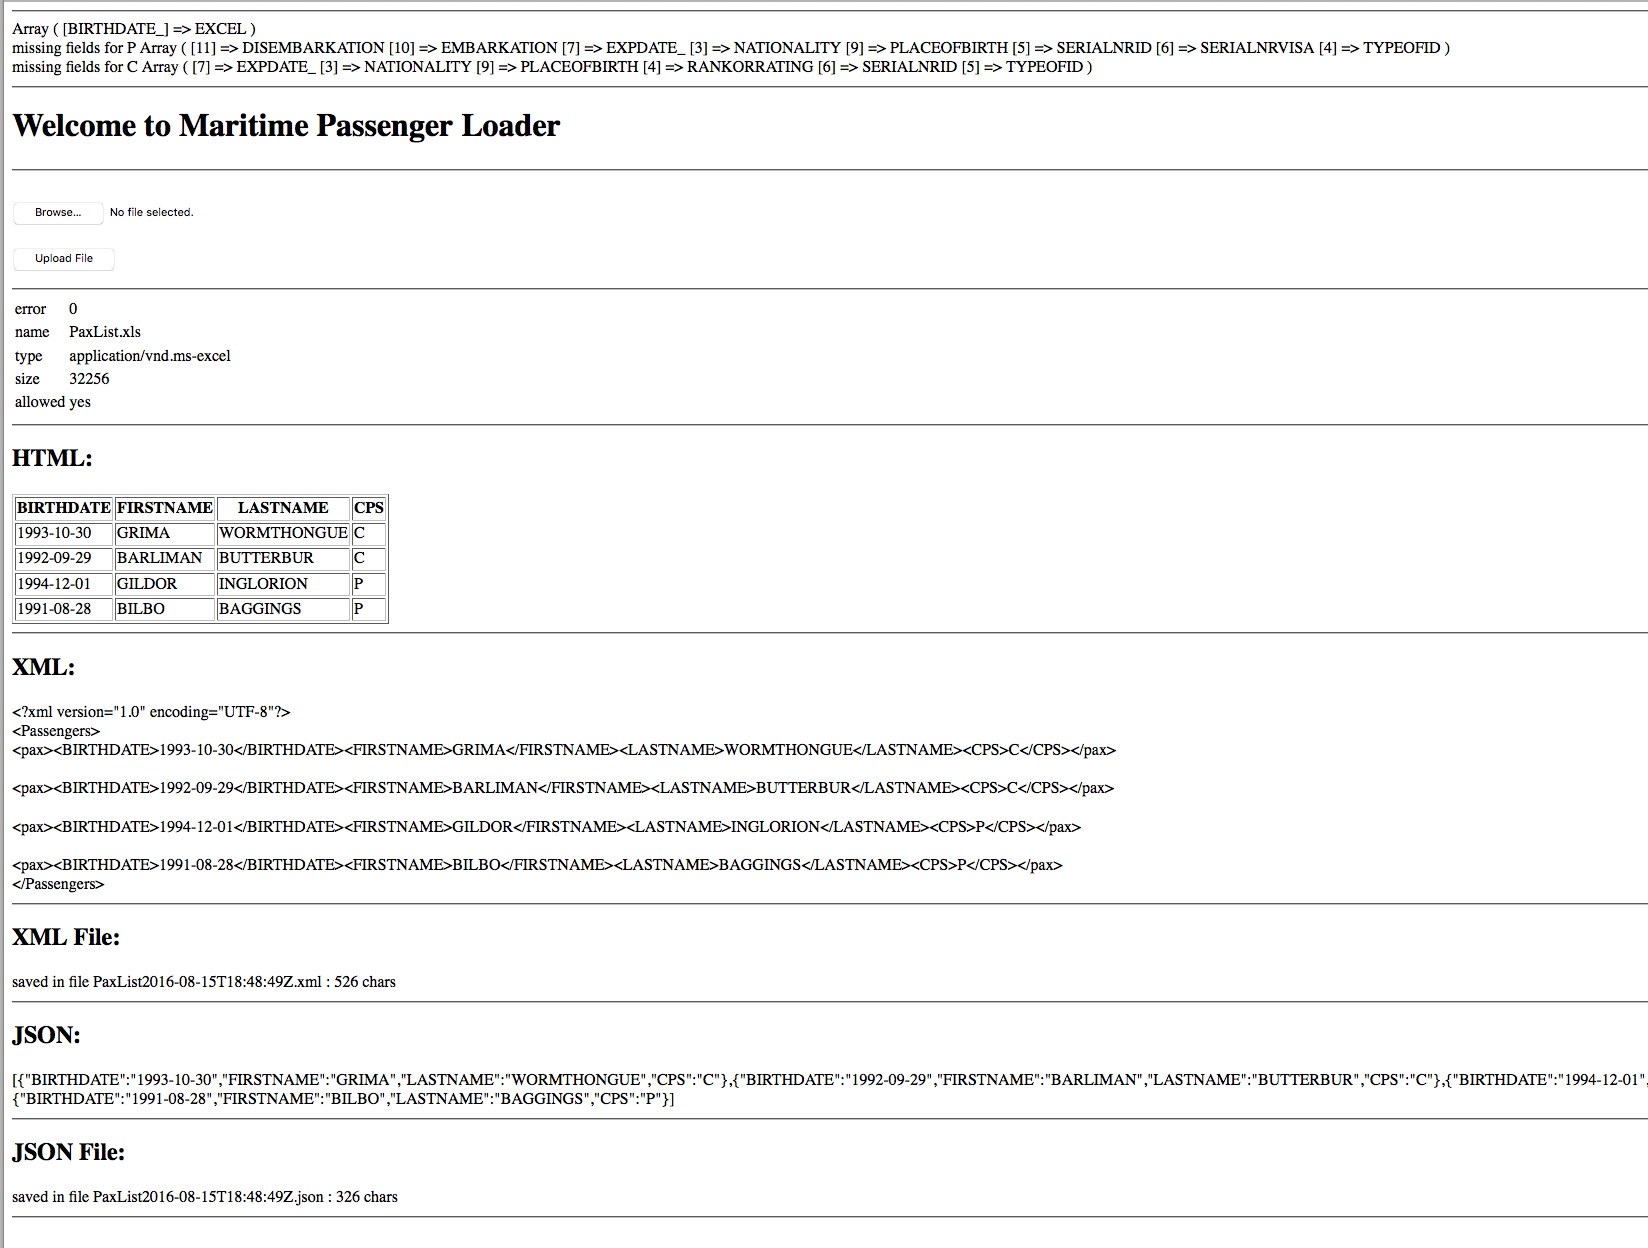
\includegraphics{figures/after}

\section{The Future}
This is much more than an invitation to collaborate. This is only a starter. There is much more to do, and we will do it altogether. We are looking, not only, for more Decoder, Filters and Encoder: we are also looking for people able to translate to other programming languages like Java, C++, Python, Objective-C, ... Let us publish our work, your work in order to avoid to reinvent the wheel. 

Make Europe a better place to live, make the Earth a better place to live.
\end{document}


